%  Rapport final – Vora H26
%  Collège Jean-de-Brébeuf, Département d'informatique
%  Arthur Girard, François Lamarre, Maxime Vanseveren

\documentclass{rapportbrebeuf}
\addbibresource{references.bib}
\usepackage{epigraph}
\usepackage{listings}
\usepackage{graphicx}
\usepackage{tikz}
\usepackage{float}
\usepackage{amsmath}
\usepackage{amsfonts}
\usepackage{amssymb}
\usepackage{geometry}

\setlength{\epigraphwidth}{0.6\textwidth}

% CHAMPS DE LA PAGE TITRE
\auteurs{Arthur \textsc{Girard}, François \textsc{Lamarre}, Maxime \textsc{Vanseveren}}
\titre{VORA}
\soustitre{RAPPORT FINAL}
\presenteA{Alexandre Desfossés Foucault}
\cours{Programmation, robotique et traitement de signal INT-SM1-24}
\groupe{Groupe 1}
\institution{Collège Jean-de-Brébeuf}
\departement{Département d'informatique}
\dateremise{8 mai 2026}

% ============================================================
\begin{document}

% Page titre, table des matières, puis début du corps
\fairePageTitre
\faireTDM
\debutCorps

% ÉPIGRAPHE
\epigraph{\textit{« L'informatique ne concerne plus les ordinateurs. Elle concerne la vie. »}}{--- \textsc{Nicholas Negroponte}, \textit{fondateur du MIT Media Lab}}
\vspace{1em}

% ABSTRACT
\section{Résumé}


\textit{Vora} est un assistant logiciel de santé visuelle utilisant la vision par ordinateur pour
prévenir les troubles liés à une exposition prolongée aux écrans. En analysant en temps réel le
ratio d'ouverture des yeux (\textit{EAR}), le programme monitore la fréquence de clignement et
automatise la règle ergonomique du 20-20-20. Cette solution non-intrusive vise à réduire la
fatigue oculaire, tout en promouvant de meilleures habitudes de travail dans l'ère du numérique. Pour assurer une fiabilité constante, l'algorithme intègre un filtrage adaptatif capable de distinguer les clignements réels des variations lumineuses ou des mouvements de l'utilisateur. L'architecture privilégie un traitement avec une base de données locale, garantissant une confidentialité absolue et une consommation énergétique optimisée sur le processeur.

% INTRODUCTION
\newpage
\section{Introduction}

L'omniprésence des outils numériques dans les environnements professionnels et académiques a transformé les habitudes de travail, mais a également engendré une hausse marquée des troubles oculaires regroupés sous le terme de syndrome de la vision artificielle ou fatigue oculaire numérique. Ce trouble se manifeste par une série de symptômes tels que la sécheresse oculaire, les maux de tête et la vision floue, affectant une proportion croissante d'utilisateurs réguliers d'écrans. La problématique centrale réside dans le fait que la concentration intense exigée par les tâches numériques inhibe le réflexe psychologique naturel du clignement, essentiel à la lubrification de la cornée et à la stabilité du film lacrymal. Cette réduction de l'activité palpébrale entraîne alors une évaporation précoce des larmes, transformant une activité quotidienne en un facteur de stress biologique significatif pour la surface oculaire.

La recherche scientifique a largement documenté ce lien de causalité, notamment à travers les travaux de Mark Rosenfield de l'Université d'État de New York. Dans sa revue intitulée \textit{Computer vision syndrome: a review of ocular causes and potential treatments}, il démontre que l'utilisation d'écrans entraîne une réduction drastique de la fréquence de clignement (pouvant chuter de près des deux tiers par rapport à la normale), ainsi qu'une augmentation préoccupante du nombre de clignements incomplets. Ces travaux soulignent que la fatigue n'est pas uniquement liée à la distance par rapport à l'écran ou à la lumière émise par les dispositifs, mais principalement à la demande cognitive élevée qui modifie le comportement biologique de l'utilisateur en retardant le déclenchement du réflexe de protection de l'oeil \cite{rosenfield2011syndrome}.

Face à ce constat, diverses stratégies préventives ont été explorées, allant de simples méthodes comme la règle du « 20-20-20 » à l'utilisation d'applications de rappel chronométrées. Cependant, la majorité des solutions existantes demeurent passives et rigides, car elles ne tiennent pas compte de la dynamique réelle du comportement visuel de l'utilisateur durant ses sessions. Le défi actuel consiste donc à concevoir des systèmes capables de monitorer intelligemment le comportement oculaire en temps réel tout en garantissant le respect de la vie privée et une intégration non-intrusive. C'est dans cette perspective d'une assistance proactive et automatisée, capable de combler l'écart entre la recommandation ergonomique et l'activité réelle, que s'inscrit le développement du projet \textit{Vora}.

% DESCRIPTION DU PROJET
\newpage
\section{Description du projet}

\textit{Vora} est conçu pour agir comme une sentinelle pour la santé oculaire des utilisateurs
d'écrans. Pour ce faire, le programme utilise un flux vidéo en direct pour calculer l'indice
d'ouverture des paupières avec un modèle pré-entraîné de MediaPipe, permettant ainsi de
comptabiliser précisément les clignements par minute. De cette façon, le logiciel permet de
compenser la baisse naturelle de ce réflexe lors d'une concentration intense devant un écran. Pour assurer la robustesse de cette détection, l'algorithme intègre un mécanisme d'adaptation dynamique : à chaque clignement confirmé, le seuil de détection est recalibré en fonction de l'amplitude des pics passés du signal \textit{EARM} (ouverture des yeux), permettant au système de s'ajuster en continu aux conditions lumineuses et à la morphologie propre de chaque utilisateur. D'ordre plus global, le fonctionnement est simple : le programme calcule une moyenne de la fréquence palpébrale et déclenche des notifications discrètes si l'hydratation oculaire est jugée insuffisante.
Parallèlement, \textit{Vora} intègre une gestion intelligente de la règle du « 20-20-20 ».
Contrairement à un simple minuteur, le décompte des vingt minutes d'activité ne progresse que si
une présence humaine est détectée devant le poste de travail. Une fois le délai atteint, l'algorithme
valide la pause seulement si l'utilisateur détourne effectivement le regard de l'écran pendant vingt
secondes, assurant ainsi une efficacité réelle de la mesure préventive. Finalement, les données de
chaque session sont condensées dans un fichier SQLite, permettant de quantifier les
bénéfices de \textit{Vora} à l'aide de graphiques mis à jour en temps réel.

Éthiquement, le respect de la vie privée constitue l'enjeu majeur de ce projet. Pour y répondre,
\textit{Vora} adopte un système de traitement 100\,\% local, faisant en sorte qu'aucune image
n'est transmise sur le réseau ou même sauvegardée sur le disque dur. Dans son ensemble, le
programme ne manipule que des vecteurs numériques issus des points de repère faciaux,
garantissant une anonymité totale et un logiciel non-intrusif.

Sur le plan environnemental, le projet vise un impact minimal en termes d'énergie et de
ressources. En effet, l'utilisation de bibliothèques optimisées comme MediaPipe permet
une exécution sur le processeur central plutôt que sur la carte graphique, réduisant
significativement la consommation électrique lors d'une utilisation prolongée. Par ailleurs, en
évitant le recours au stockage de données volumineuses ou à des services dans le nuage
(utilisation d'un modèle pré-entraîné local), \textit{Vora} minimise l'empreinte carbone liée au
transfert et à la conservation de données inutiles. 

% LOGIQUE DU CODE ET RÉPARTITION
\newpage
\subsection{Logique du code}

% Flowchart programmé avec Gemini à partir du code Mermaid original (dans le PowerPoint)
\begin{figure}[H]
    \centering
    \resizebox{0.99\textwidth}{!}{%
    \begin{tikzpicture}[
        % Définition des couleurs
        define color/.code 2 args={\definecolor{#1}{HTML}{#2}},
        define color={startfill}{E8F0FE},
        define color={startstroke}{2B5C8F},
        define color={uifill}{FFFFFF},
        define color={uistroke}{2B5C8F},
        define color={logicfill}{F8F9FA},
        define color={logicstroke}{6C757D},
        define color={timerfill}{FFF8E1},
        define color={timerstroke}{BCAAA4},
        define color={dbfill}{E8F5E9},
        define color={dbstroke}{81C784},
        define color={alertfill}{FFEBEE},
        define color={alertstroke}{E57373},
        %
        % Styles de base (Serif pour matcher le document)
        base/.style={align=center, font=\small, inner xsep=10pt, inner ysep=8pt, minimum width=3.4cm, minimum height=1.2cm},
        start/.style={base, rectangle, rounded corners=3mm, draw=startstroke, fill=startfill, thick},
        ui/.style={base, rectangle, draw=uistroke, fill=uifill, thick},
        logic/.style={base, rectangle, draw=logicstroke, fill=logicfill, thick},
        timer/.style={base, rectangle, draw=timerstroke, fill=timerfill, thick},
        alert/.style={base, rectangle, draw=alertstroke, fill=alertfill, thick},
        database/.style={base, cylinder, shape border rotate=90, aspect=0.25, draw=dbstroke, fill=dbfill, thick, minimum width=4.5cm, minimum height=2.2cm, inner ysep=16pt},
        dbbox/.style={base, rectangle, draw=dbstroke, fill=dbfill, thick},
        %
        % Styles des lignes
        line/.style={draw, -Latex, thick, color=black!80},
        dashedline/.style={draw, -Latex, thick, dashed, color=black!60},
        %
        % Style pour les étiquettes de section (Noir et lisible)
        section label/.style={font=\Large\bfseries\color{black}, align=left}
    ]
    %
    % ================= NIVEAU 1 : NAVIGATION =================
    \node[start] (A)  at (0, 0)      {Lancement de Vora};
    \node[ui]    (B)  at (0, -2.2)   {Interface Flet};
    \node[ui]    (C)  at (-3.5, -5.0) {Section\\Démarrage};
    \node[ui]    (D)  at (3.5, -5.0)  {Section\\Analyse};
    %
    % ================= NIVEAU 2 : LOGIQUE DE VISION =================
    \node[start] (E)  at (-3.5, -8.0) {Action : Lancer};
    \node[logic] (F)  at (-3.5, -10.0) {Thread Backend\\(Asynchrone)};
    \node[logic] (G)  at (-3.5, -12.0) {Capture Vidéo\\+ MediaPipe};
    %
    \node[logic] (H)  at (-8.0, -16.5) {Calcul EAR\\\& Clignements};
    \node[alert] (M)  at (-3.5, -16.5) {Analyse fatigue :\\Avertissement sécheresse};
    \node[timer] (L)  at (1.5, -16.5)  {ErgoTimer :\\Présence \& pauses};
    %
    % ================= NIVEAU 3 : SORTIE DE DONNÉES =================
    \node[database] (I) at (-3.5, -21.5) {Base de données SQLite};
    \node[logic]    (J) at (3.5, -21.5)  {Flux vidéo\\en temps réel};
    \node[dbbox]    (K) at (0, -25.5)    {Graphiques de\\fréquences et sessions};
    %
    % ================= BRACKETS ET ÉTIQUETTES (NOIR) =================
    % Position X de l'accolade, repoussée pour éviter tout overlap
    \def\Xbrace{7.0} 
    %
    % NAVIGATION (sans 'mirror' pour pointer vers la droite)
    \draw [decorate, decoration={brace, amplitude=12pt}, thick, color=black] 
        (\Xbrace, 0.8) -- (\Xbrace, -6.0) 
        node [midway, right=15pt, section label] {NAVIGATION};
    %
    % LOGIQUE DE VISION
    \draw [decorate, decoration={brace, amplitude=12pt}, thick, color=black] 
        (\Xbrace, -7.0) -- (\Xbrace, -18.0) 
        node [midway, right=15pt, section label] {LOGIQUE DE\\VISION};
    %
    % SORTIE DE DONNÉES
    \draw [decorate, decoration={brace, amplitude=12pt}, thick, color=black] 
        (\Xbrace, -19.5) -- (\Xbrace, -27.0) 
        node [midway, right=15pt, section label] {SORTIE DE\\DONNÉES};
    %
    % ================= CONNEXIONS SOLIDES =================
    \draw[line] (A) -- (B);
    \draw[line, rounded corners] (B.south) -- (0, -3.6) -| (C.north);
    \draw[line, rounded corners] (B.south) -- (0, -3.6) -| (D.north);
    %
    \draw[line] (C) -- (E);
    \draw[line] (E) -- (F);
    \draw[line] (F) -- (G);
    %
    % Bus principal sortant de Capture Vidéo (Y = -14.2)
    \draw[line, rounded corners] (G.south) -- (-3.5, -14.2) -| (H.north);
    \draw[line, rounded corners] (G.south) -- (-3.5, -14.2) -| (L.north);
    \draw[line, rounded corners] (G.south) -- (-3.5, -14.2) -| (J.north);
    %
    \draw[line] (H.east) -- (M.west);
    %
    \draw[line, rounded corners] (H.south) |- (I.west);
    \draw[line]                  (M.south) -- (I.north);
    \draw[line, rounded corners] (L.south) |- (I.east);
    %
    \draw[line, rounded corners] (I.south) |- (K.west);
    %
    % ================= CONNEXIONS POINTILLÉES =================
    % C vers M : descente protégée à X=-0.85 (pile au centre, loin de la boîte rouge)
    \draw[dashedline, rounded corners] (C.east) -- (-0.85, -5.0) -- (-0.85, -15.2) -| (M.north);
    %
    % Prolongation de la ligne entre les boîtes vers Flux Vidéo
    \draw[dashedline, rounded corners] (-0.85, -15.2) -- (-0.85, -19.0) -| ([xshift=-15pt]J.north);
    %
    % D vers K : Contournement extérieur à X=6.0 (bien avant le bracket)
    \draw[dashedline, rounded corners] (D.east) -- (6.0, -5.0) |- (K.east);
    %
    \end{tikzpicture}%
    }
    \caption{Schéma de la logique globale du code\protect\footnotemark}
    \label{fig:logique_code}
\end{figure}
\footnotetext{Schéma converti de Mermaid à TikZ avec l'aide de Gemini.}

\newpage
\subsection{Répartition du travail}

\subsubsection{Arthur Girard}

Dans la conception de \textit{Vora}, Arthur a principalement travaillé sur le traitement des données renvoyées par MediaPipe. Essentiellement, il a pris la charge de l'implémentation de la logique pour l'\textit{EAR} (s'inspirant d'un dépôt GitHub similaire \cite{github2024eyeblink}), en s'occupant également du filtrage des signaux pour assurer une détection des clignements efficace et optimisée. Par ailleurs, Arthur a aussi conçu toute la machine à états et le système de minuteurs intelligents derrière l'automatisation de la règle ergonomique du 20-20-20. Finalement, celui-ci a également contribué à l'intégration des algorithmes d'arrière-plan dans l'interface utilisateur, fournissant l'idée et le code derrière la transmission du flux OpenCV à l'onglet principal du logiciel.

\subsubsection{François Lamarre}

Dans la conception de Vora, Francois a principalement travaillé sur l’extraction des données à l’aide de la librairie MediaPipe. Cette extraction avait comme rôle d’extraire une liste de dictionnaires retournant les coordonnées des points sur le visage. Par ailleurs, celui-ci a également conçu le système derrière la gestion des données, en créant la base de données SQLite3 et la gestion de celle-ci.  

\subsubsection{Maxime Vanseveren}

Maxime a principalement été responsable de la confection de l’interface graphique avec la bibliothèque Flet. Avec l’aide d’Arthur, Maxime a aussi fusionné l’algorithme d’arrière-plan (backend) a l’interface utilisateur (frontend) à l’aide de la librairie base64, permettant l’affichage en temps réel des graphiques et de la caméradans les onglets « Analyse » et « Démarrage » respectivement. 

% RECHERCHES INDIVIDUELLES
\newpage
\section{Recherches individuelles}

\subsection{L'efficacité du filtre à différences de moyennes mobiles (Arthur Girard)}

Dans \textit{Vora}, la vision par ordinateur (OpenCV et MediaPipe) analyse le comportement des paupières en temps réel. Toutefois, les données brutes extraites sont soumises à un bruit environnemental important (grain du capteur, micromouvements, variations d'éclairage). Un simple seuil fixe étant inefficace face aux variations morphologiques et lumineuses, le logiciel nécessite un mécanisme d'isolation adaptatif pour distinguer un clignement physiologique du bruit de fond : le filtrage par double moyenne mobile (\textit{EARM}).

Dans les faits, l'enjeu majeur de \textit{Vora} est de distinguer un événement provoqué par un
réflexe d'un bruit de fond aléatoire. Un simple seuil fixe sur l'ouverture de l'œil ne suffit pas,
car la morphologie de chaque utilisateur et les conditions lumineuses varient constamment. Il est
donc nécessaire de mettre en œuvre un mécanisme d'isolation mathématique capable de s'adapter
dynamiquement à ces variations.

Ainsi, cette recherche s'articulera autour de la question suivante :

\begin{quote}
  \raggedright
  \textit{Comment l'utilisation d'un filtre à différence de moyennes mobiles permet-elle d'isoler
  mathématiquement des signaux physiologiques en vision par ordinateur ?}
\end{quote}

Avant d'isoler le signal, il faut définir la métrique source. \textit{Vora} utilise l'\textit{Eye
Aspect Ratio} (\textit{EAR}), une valeur scalaire calculée à partir de six points de repère faciaux
entourant chacun des yeux. Pour chaque œil, l'\textit{EAR} est calculé selon la formule suivante :
\[
  EAR = \frac{\lVert p_2 - p_6 \rVert + \lVert p_3 - p_5 \rVert}{2\,\lVert p_1 - p_4 \rVert}
\]
Où $p_n$ représente les coordonnées 3D des points extraits par MediaPipe. Bien que la formule originale de Soukupová et Čech ait été développée en deux dimensions \cite{soukupova2016real}, MediaPipe Face Mesh fournit des coordonnées 3D pour chaque point de repère facial, auxquelles la norme euclidienne s'applique directement sans modification de la formule. L'\textit{EAR} quantifie le degré d'ouverture de l'œil : il est stable lorsque l'œi est ouvert (environ 0,3) et chute rapidement vers 0 lors d'un clignement \cite{soukupova2016real}.

Toutefois, l'\textit{EAR} n'est jamais un signal « propre ». Il intègre du bruit haute fréquence (imprécisions du capteur) et subit une dérive basse fréquence (changements de posture) qui modifie sa valeur de base indépendamment des clignements réels.

La solution retenue dans \textit{Vora} pour répondre à cette problématique est le filtre
\textit{EARM}, qui repose sur une différence de moyennes mobiles (\textit{Difference of Moving
Averages -- DoMA}). Pour ce faire, le système maintient deux moyennes mobiles simples
(\textit{Simple Moving Average -- SMA}) calculées en parallèle sur un tampon d'historique.
Effectivement, une moyenne « lente » (30 frames) agit comme ligne de base dynamique pour capturer la tendance de fond, tandis qu'une moyenne « rapide » (3 frames) suit les variations immédiates en lissant le grain du capteur. L'isolation du signal de clignement est alors définie par la différence entre les deux moyennes :
\[
  EARM = SMA_{lente} - SMA_{rapide}
\]
Mathématiquement, cette soustraction annule les composantes communes aux deux fenêtres. En
effet, si l'utilisateur penche la tête lentement, les deux moyennes varient de la même manière et
leur différence reste proche de zéro. En revanche, lors d'un clignement, la chute de l'\textit{EAR}
est si rapide que seule la moyenne rapide la détecte immédiatement. La moyenne lente reste « en
retard » sur son niveau haut, créant un pic massif dans l'\textit{EARM} et permettant une
détection fiable \cite{kuwahara2022eye}.

Pour comprendre l'efficacité de cette méthode, il faut examiner les propriétés de la moyenne mobile à travers les travaux de Steven W. Smith. Dans le chapitre 15 de son ouvrage \textit{The Scientist and Engineer's Guide to Digital Signal Processing} \cite{smith1997guide}, Smith démontre que la moyenne mobile est le filtre linéaire optimal pour une tâche fondamentale en vision par ordinateur : réduire le bruit tout en préservant la netteté d'une montée ou d'une chute brute du signal : 

\begin{figure}[H]
    \centering
    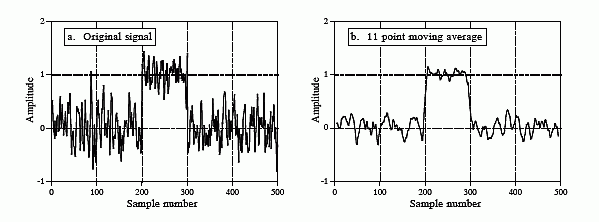
\includegraphics[width=0.8\textwidth]{figure_smith_15_1.png}
    \caption{On observe qu'une fenêtre plus large réduit davantage le bruit mais dégrade la netteté des fronts. La moyenne mobile constitue la solution optimale pour minimiser le bruit tout en préservant la réponse à l'échelon. Figure extraite et adaptée du chapitre 15 de \cite{smith1997guide}.}
    \label{fig:smith_phase}
\end{figure}

Pour Vora, cela signifie que la moyenne mobile est le filtre le plus performant pour cette tâche spécifique, soit supprimer le grain de l'image sans « arrondir » la chute de l'\textit{EAR}, permettant ainsi de capturer l'instant exact du clignement. Cette optimalité est toutefois à entendre dans un sens précis, car la moyenne mobile minimise le bruit résiduel à nombre de points fixe tout en préservant la netteté des fronts du signal, ce qui en fait le choix le mieux adapté à la détection de clignements, sans pour autant constituer le filtre optimal au sens large du traitement de signal. En effet, Smith explique que ce filtre est médiocre dans le domaine fréquentiel pur, car sa réponse en fréquence suit une fonction \textbf{sinc} discrète présentant une atténuation très lente des fréquences indésirables : 
\[
  \lvert H(e^{jw}) \rvert = \frac{1}{M} \left| \frac{\sin(\omega M/2)}{\sin(\omega /2)} \right|
\]
C'est ici que réside la pertinence du filtre DoMA de Vora, car en utilisant la différence de ces deux fonctions, on compense la faiblesse naturelle de la moyenne mobile dans le domaine des fréquences. En fait, on transforme deux filtres « médiocres » en une fenêtre de transmission plus sélective (un filtre passe-bande) qui rejette le courant continu (DC) lié à la posture et les hautes fréquences liées au bruit du capteur. Ce qui subsiste dans le signal \textit{EARM} est précisément le signal physiologique pur, centré autour de la fréquence naturelle des clignements humains.

Cette isolation spectrale est renforcée par une propriété fondamentale des filtres à moyenne mobile : la linéarité de phase. Contrairement aux filtres à réponse impulsionnelle infinie (IIR) comme le filtre de Butterworth, la moyenne mobile ne déforme pas le signal temporellement. Un filtre de Butterworth peut introduire des déphasages non linéaires qui déplacent les composantes fréquentielles les unes par rapport aux autres, ce qui risquerait de distordre la forme du clignement \cite{smith1997guide}. Pour une application comme Vora, cela signifie que le début et la fin exacts du mouvement des paupières sont préservés mathématiquement, ce qui est indispensable pour une analyse fine de la fatigue.

Le tout permet alors enfin de transformer une détection statique en un processus
dynamique et adaptatif. Puisque l'\textit{EARM} est recentré autour de zéro par la soustraction de
la moyenne lente, le système peut appliquer un seuil de détection relatif plutôt qu'absolu. Dans le
code de Vora, cette isolation est exploitée par une boucle de rétroaction qui analyse les pics de
signal des clignements passés pour ajuster le seuil de détection en temps réel. Cette capacité
d'adaptation montre alors bien comment le filtre DoMA permet à l'algorithme de comprendre
l'écart entre un état stable (œil ouvert) et une impulsion physiologique (clignement) à travers le
bruit environnemental.

En conclusion, l'utilisation d'un filtre à différence de moyennes mobiles offre une solution
robuste au paradoxe de la vision par ordinateur : obtenir une précision biologique à partir de
capteurs imparfaits. En isolant la différence entre une tendance lente et une dynamique plus
rapide, le filtre DoMA retire les artefacts pour ne laisser que l'essence du
mouvement physiologique, garantissant ainsi la fiabilité de la surveillance de la fatigue oculaire.

\newpage
\subsection{Fonctionnement de MediaPipe (François Lamarre)}

Le problème de la détection des points de repère faciaux (Landmarks) en vision par ordinateur a été abordé de multiples manières au cours des trente dernières années. Avant l'émergence des réseaux de neurones, une approche courante pour identifier des objets ou le corps humain reposait sur les structures picturales, qui modélisaient les formes par un assemblage de parties déformables (souvent représentées par des rectangles). Cette méthode s'est toutefois révélée inefficace pour la détection faciale, car elle manquait de la précision nécessaire pour localiser des points dans des zones exigeant une grande précision, comme le contour des yeux ou des paupières.

L'essor des réseaux de neurones, et particulièrement des réseaux de neurones convolutifs (CNN), a permis d'augmenter significativement la précision de ces détections. Notamment, le modèle Face Mesh de Google permet d’identifier plus de 468 points sur le visage. Bien que des nouvelles versions porte des grandes améliorations, ce rapport se concentrera sur le modèle de base, détaillé dans l'étude Real-time Facial Surface Geometry from Monocular Video on Mobile GPUs.\newline
Le modèle peut être séparé en plusieurs étapes :

\begin{enumerate}
    \item Le flux vidéo est d’abord traité par BlazeFace, un détecteur de visage ultra-léger basé sur une architecture SSD (Single Shot Multi Box Detector). Son rôle est d'identifier la boîte englobante (bouding box) du visage pour isoler la région d'intérêt (ROI)
    \item Recadrage: pour que le système ne soit pas perturbé par les mouvements de l'utilisateur, il se corrige. Chaque fois que le visage est éloigné de la caméra, cette étape permet de redimensionner le visage détecté. Cette étape revient donc à changer le référentiel pour s'adopter à la position du visage.
    \item Estimation des coordonnées par un Réseau Résiduel (Facemesh): Le visage aligné est ensuite passé à travers un réseau de régression résiduel. Cette architecture utilise des blocs de convolution avec des connexions sautés (skip connections) pour prédire directement les coordonnées des 468 points 3D.
    \item Boucle de rétroaction (mise à jour du ROI): Pour optimiser les performances en temps réel, le modèle utilise les points prédits à l'image précédente pour mettre à jour la région d'intérêt de l'image suivante. Cela permet de sauter l'étape de détection (BlazeFace)sur la majorité des images, en tant que le visage reste dans le champs de vision de la caméra.
\end{enumerate}

Alors, la question pour cette section du rapport est : « Comment les réseaux de neurones (CNN et ResNet) permettent-ils à MediaPipe d'analyser des images et retourner les points sur le visage avec précision? »

Tout d’abord, il faut comprendre pourquoi un réseau résiduel (ResNet) est important. Dans un réseau de neurones, il serait intuitif de penser que plus il possède de couches, plus il devient performant, car l’ajout de poids permettrait d’améliorer la précision ou l’efficacité du modèle. Cependant, rajouter plus de couches peut mener à une dégradation des performances. En effet, cela n'est pas dû au surapprentissage (overfitting), mais bien à la complexité derrière l’optimisation de modèles massifs.Dans un réseau de neurones de base, si on veut mettre à jour les poids ($w$), on utilise la descente de gradient afin de minimiser le coût. Dans un réseau très profond, à force de faire des multiplications successives, le gradient devient tellement petit que la mise à jour des poids est presque invisible. Un ResNet règle donc ce problème de « Vanishing gradient ».

Soit un réseau de neurones profonds classique (sans ResNet) composé de $L$ couches successives, où chaque couche n'a qu'un seul neurone (exemple simplifié).

Soient :
\[ a_i = \sigma(z_i) \quad \text{où} \quad z_i = w_i \cdot a_{i-1} + b \]

Où $\sigma$ est la fonction d'activation (ex: ReLU).
\[ a_i = f(z_i) \quad \text{où} \quad z_i = w_i \cdot a_{i-1} + b \]


Notons la dérivée partielle pour une couche :
$$\frac{\partial a_i}{\partial a_{i-1}} = \frac{\partial \sigma(z_i)}{\partial a_{i-1}} + \frac{\partial a_{i-1}}{\partial a_{i-1}} = (\sigma^\prime(z_i) \cdot w_i)$$

Alors, pour un réseau de $L$ couches, le gradient par rapport aux premiers poids $w_1$ suit la règle de dérivation en chaîne:

\[ \frac{\partial C}{\partial w_1} = \frac{\partial C}{\partial a_L} \cdot \frac{\partial a_L}{\partial a_{L-1}}  \cdot \dots \cdot  \frac{\partial a_{2}}{\partial a_1}  \cdot \frac{\partial a_1}{\partial w_1}\]

En remplaçant chaque terme $\frac{\partial a_i}{\partial a_{i-1}}$ par sa valeur calculée ($w_i \cdot \sigma^\prime(z_i)$), on obtient
$$ \frac{\partial C}{\partial w_1} = \frac{\partial C}{\partial a_L} \cdot (w_L \cdot \sigma^\prime(z_L)) \cdot \dots \cdot (w_2 \cdot \sigma^\prime(z_2)) \cdot \frac{\partial a_1}{\partial w_1} $$

$$ \frac{\partial C}{\partial w_1} = \frac{\partial C}{\partial a_L} \cdot \left( \prod_{i=2}^{L} \sigma^\prime(z_i) \cdot w_i \right) \cdot \frac{\partial a_1}{\partial w_1} $$

Prenons commme exemple la fonction d'activation ReLU :
\[ \sigma(z) = \max(0, z) \]
Sa dérivée est définie par :
\[ f^\prime(z) = 
\begin{cases} 
1 & \text{si } z > 0 \\
0 & \text{si } z \leq 0
\end{cases} \]

Si l'initialisation des poids $w_i \approx 0,5$, et que le réseau admet des valeurs positives ($z > 0$), le produit devient :

\[ (0,5 \cdot 1) \cdot (0,5 \cdot 1) \cdot \dots \]

Posons que $L=50$ couches (ou un réseau de neurone profond quelconque) :

\[ \frac{\partial C}{\partial w_1} = \frac{\partial C}{\partial a_L} \cdot (0,5)^{49} \cdot \frac{\partial a_1}{\partial w_1} \]

Le gradient \textbf{"disparaît"}, il devient une valeur minime : 
\[ (0,5)^{49} \approx 10^{-15} \]

Lorsqu'on met à jour $w_1$, il n'y a presque pas de différence. Le gradient devient "invisible" :
\[ w_{\text{nouveau}} = w_1 - \alpha \frac{\partial C}{\partial w_1} \approx w_1 - \alpha \cdot 10^{-15} \]
Bien que cela soit un exemple simplifié, pour un réseau de neurone à plusieurs couches et poids, il est entièrement possible que le gradient "disparaisse" lorsqu'il dérive par rapport à un poids loin dans le réseau. Alors, comment un réseau de neurone résiduel permet d'éviter ce problème ? Voici un schéma simplifié d'un réseau de neurone résiduel :

% --- STYLES RÉSEAU RÉSIDUEL ---
\definecolor{cyan_custom}{RGB}{0, 188, 212}
\definecolor{pink_custom}{RGB}{233, 30, 99}
\definecolor{yellow_custom}{RGB}{255, 193, 7}
\definecolor{red_sum}{RGB}{211, 47, 47}

\tikzset{
    base_rect/.style={rectangle, draw=black, thick, text centered, font=\sffamily\tiny\bfseries, rounded corners=2pt},
    layer_box/.style={base_rect, fill=cyan_custom!30, minimum width=1cm, minimum height=1.4cm},
    small_box/.style={base_rect, fill=gray!20, minimum width=1cm, minimum height=0.7cm},
    relu_box/.style={base_rect, fill=pink_custom!30, minimum width=0.8cm, minimum height=0.7cm},
    sum/.style={circle, draw=red_sum, fill=red_sum!20, thick, minimum size=0.5cm, font=\sffamily\small, inner sep=0pt}
}

\begin{figure}[H]
    \centering
    \begin{tikzpicture}[node distance=1cm, >=Stealth]

    % Noeuds
    \node (In) [small_box, fill=yellow_custom!30] {Entrée ($x$)};
    \node (L1) [layer_box, right=of In] {\rotatebox{90}{Couche 1}};
    \node (R1) [relu_box, right=of L1] {ReLU};
    \node (L2) [layer_box, right=of R1] {\rotatebox{90}{Couche 2}};
    \node (S1) [sum, right=of L2] {+};
    \node (Out) [small_box, fill=yellow_custom!30, right=of S1] {Sortie $h(x)$};

    % Flèches du chemin principal
    \draw [->, thick] (In) -- (L1);
    \draw [->, thick] (L1) -- (R1);
    \draw [->, thick] (R1) -- (L2);
    \draw [->, thick] (L2) -- node[above, font=\tiny\itshape] {$f(x)$} (S1);
    \draw [->, thick] (S1) -- (Out);

    % Skip Connection (Le saut)
    \draw [->, thick, draw=medblue] (In.east) -- ++(0.3, 1.1) -| node[pos=0.25, above, font=\tiny\sffamily\bfseries] {Skip Connection ($x$)} (S1.north);

    % Équation sous le bloc
    \node[below=0.4cm of S1, font=\sffamily\tiny] {$h(x) = f(x) + x$};
    
    \end{tikzpicture}
    \caption{Unité résiduelle compacte (ResNet).}
\end{figure}

Ce schéma représente un bloc résiduel. C'est ce mécanisme qui permet d'entraîner des réseaux de neurones profonds sans perdre le signal du gradient. L'entrée $x$ traverse d'abord les couches de calcul. Ce qui est retourné à la fin de ce parcours est la fonction résiduelle $f(x)$.La flèche supérieure représente le saut de connection. C'est la "skip connection". L'entrée $x$ est copiée et "saute" les couches de calcul pour être ajoutée directement plus loin. La sortie finale est donc l'addition des deux chemins :
\[ h(x) = f(x) + x \]

Pour entraîner le réseau, on calcule la dérivée de la sortie par rapport à l'entrée. Si on applique la dérivée de l'équation $h(x) = f(x) + x$ :
\[ \frac{{d}h(x)}{{d}x} = \frac{{d}f(x)}{{d}x} + \frac{{d}x}{{d}x} = f^\prime(x) + 1 \]

Si nous reprenons l'exemple donné pour le problème du gradient qui disparaît, on remarque donc que le terme $+1$ permet de garantir que le gradient ne sera jamais inférieur à 1 comme le montre l'équation suivante : 
\[ \frac{\partial C}{\partial w_1} = \frac{\partial C}{\partial a_L} \cdot (w_L \cdot f^\sigma(z_L) + 1) \cdot \dots \cdot (w_2 \cdot f^\sigma(z_2) + 1) \cdot \frac{\partial a_1}{\partial w_1} \]

Lors de la rétropropagation, le gradient évite donc de s'annuler dans des multiplications de petites valeurs. La skip connection crée un lien direct qui permet aux premières couches de recevoir un signal clair pour mettre à jour leurs poids, peu importe la profondeur du réseau.

% \break
% \begin{figure}
%     \centering
%     \includegraphics[width=0.9\linewidth]{convolution.png}
%     \caption{Exemple de convolution}
%     \label{fig:placeholder}
% \end{figure}
\usetikzlibrary{matrix, positioning, arrows.meta}
\begin{figure}[htbp]
    \begin{tikzpicture}[
        cell/.style={rectangle, draw=black, minimum size=8mm, anchor=center},
        input_color/.style={fill=blue!10},
        kernel_color/.style={fill=red!20},
        output_color/.style={fill=green!10},
        highlight/.style={draw=red, line width=1.5pt}
    ]
    
    % --- INPUT TENSOR (3x3) ---
    \matrix (input) [matrix of nodes, nodes={cell, input_color}, column sep=-\pgflinewidth, row sep=-\pgflinewidth] {
        5 & 2 & 1 \\
        0 & 4 & 2 \\
        3 & 1 & 6 \\
    };
    \node[above=5pt of input] {\textbf{Input Tensor (3x3)}};
    
    % Encadrement de la zone de convolution (les 4 premières cellules)
    \draw[highlight] (input-1-1.north west) rectangle (input-2-2.south east);
    
    % --- KERNEL (2x2) ---
    \matrix (kernel) [matrix of nodes, nodes={cell, kernel_color}, column sep=-\pgflinewidth, row sep=-\pgflinewidth, right=2cm of input] {
        1 & 0 \\
        0 & 1 \\
    };
    \node[above=5pt of kernel] {\textbf{Kernel (2x2)}};
    
    % --- FEATURE MAP / OUTPUT (2x2) ---
    \matrix (output) [matrix of nodes, nodes={cell, output_color}, column sep=-\pgflinewidth, row sep=-\pgflinewidth, right=2cm of kernel] {
        9 & 4 \\
        1 & 10 \\
    };
    \node[above=5pt of output] {\textbf{Feature Map (2x2)}};
    
    % --- CONNEXIONS / FLÈCHES ---
    \draw[-{Stealth[scale=1.2]}, thick] (input) -- (kernel) node[midway, above] {$\ast$};
    \draw[-{Stealth[scale=1.2]}, thick] (kernel) -- (output) node[midway, above] {$=$};
    
    \end{tikzpicture}
    \caption{Exemple de convolution à partir d'un tenseur 3x3}
    \label{fig:schema_convolution}
\end{figure}


Une image est composée de plusieurs pixels ayant chacun une valeur d’intensité. Prenons l’exemple de la figure 3 où l’entrée est une image et où nous effectuons une convolution :L’astérisque ($*$) représente l’opération de convolution. Le noyau (ou kernel) agit comme une fenêtre glissante qui parcourt l’image d’entrée pour en extraire des caractéristiques. Comme illustré en bleu, chaque valeur de la matrice de sortie est égale à la somme des produits élément par élément des cases respectives :

\begin{enumerate}
    \item \textbf{En haut à gauche :} $(1 \cdot 1) + (2 \cdot 0) + (4 \cdot 0) + (5 \cdot 1) = 6$
    \item \textbf{En haut à droite :} $(2 \cdot 1) + (3 \cdot 0) + (5 \cdot 0) + (6 \cdot 1) = 8$
    \item \textbf{En bas à gauche :} $(4 \cdot 1) + (5 \cdot 0) + (7 \cdot 0) + (8 \cdot 1) = 12$
    \item \textbf{En bas à droite :} $(5 \cdot 1) + (6 \cdot 0) + (8 \cdot 0) + (9 \cdot 1) = 14$
\end{enumerate}

Note : Cet exemple est grandement inspiré de l'article de Jorge Cardete sur Medium : « Convolutional Neural Networks: A Comprehensive Guide ».


Lors de l'analyse d’une image, plusieurs noyaux ou « filtres » sont appliqués. Ces filtres correspondent aux poids ($w$) du réseau de neurones. Chaque filtre génère une carte de caractéristiques (feature map) qui est ensuite transmise aux couches suivantes. Dans un contexte plus concret, les filtres vont permettent de trouver des caractéristiques dans une image, par exemple de déterminer le contour d'une personne. La matrice d'entrée peut également inclure du remplissage (padding), consistant à ajouter des zéros sur le contour pour éviter que le noyau ne néglige les valeurs dans les coins. De plus, le noyau peut avoir un pas (stride) différent, déterminant de combien de cases la fenêtre glisse à chaque étape (par exemple, un bond de 1 ou 2 pixels). En résumé, le but d’une couche de convolution est d'extraire des motifs ou des caractéristiques à partir de données d’entrée. Les données produites peuvent ensuite être « aplaties » (flatten) en un vecteur à une dimension pour être traitées par des couches connectées.

Lorsqu'une couche convolutive va sortir ses données, elle peut non seulement être sortit dans un vecteur à une dimensions, mais également sous forme de tenseur pour passer à travers une fonction d'acitvation commme ReLu.
Alors, un ResNet peut contenir des couches de convolution avec des fonction d'activaiton ReLu, ce qui va permettre de faire des "saut" de connections pour les gradients.
Dans le cas de la librairie Mediapipe, voici comment le modèle Facemesh permet d'intégrer ces deux types de réseaux de neurones.


\begin{enumerate}
    \item Les tenseurs provenant d'une image sont rapidement réduits à l'aide de couches convolutives. Ce processus est agressif afin de réduire les données du tenseur en des données qui représente une fonctionnalité. Par exemple,le contour autour des yeux.
    \item Les données sont ensuite passé dans des bloc résiduel qui permettent un réseau de neurone extrêmement profond sans avoir ce soucié des problèmes de gradient qui disparaît.
    \item Finalement, dans les dernières couche du réseau, un problème de régression est résout afin de retourner les coordonnées des points sur le visage de l'utilisateur.
\end{enumerate}

\definecolor{codegreen}{rgb}{0,0.6,0}
\definecolor{codegray}{rgb}{0.5,0.5,0.5}
\definecolor{codepurple}{rgb}{0.58,0,0.82}
\definecolor{backcolour}{rgb}{0.95,0.95,0.92}
\definecolor{medblue}{rgb}{0.0,0.45,0.74}
\lstdefinestyle{mystyle}{
    backgroundcolor=\color{backcolour},   
    commentstyle=\color{codegreen},
    keywordstyle=\color{magenta},
    numberstyle=\tiny\color{codegray},
    stringstyle=\color{codepurple},
    basicstyle=\ttfamily\footnotesize,
    breakatwhitespace=false,         
    breaklines=true,                 
    captionpos=b,                    
    keepspaces=true,                 
    numbers=left,                    
    numbersep=5pt,                  
    showspaces=false,                
    showstringspaces=false,
    showtabs=false,                  
    tabsize=2
}
\lstset{style=mystyle}
% Bibliothèques TikZ essentielles
\usetikzlibrary{calc, positioning, shapes.geometric, arrows.meta, fit, backgrounds}

La figure 5 montre un petit code python qui permet simplifier la logique du réseau de neurone de FaceMesh lors d'une propagation vers l'avant.

\textbf{Explication du code :}
\begin{enumerate}
    \item \textbf{Importation :} On importe la librairie TensorFlow qui permet de créer et d'entraîner des réseaux de neurones.
    \item \textbf{Entrée :} Initialisation de la variable d'entrée. Elle reçoit l'image en format $64 \times 64$ pixels.
    \item \textbf{Convolutions agressives :}
    \begin{itemize}
        \item \textbf{Première couche :} Elle reçoit l'image et applique $32$ filtres de taille $3 \times 3$. Ensuite, la fonction d'activation {ReLU} est appliquée sur tous les éléments.
        \item \textbf{Deuxième couche :} Le nouveau tenseur passe par une autre convolution avec $64$ filtres de taille $3 \times 3$.
    \end{itemize}
    \item \textbf{Bloc résiduel :} Ce bloc effectue une convolution et additionne l'entrée au résultat ($h(x) = f(x) + x$). Cela permet de garder l'information d'origine à travers les couches.
    \item \textbf{Régression finale :}
    \begin{itemize}
        \item \textbf{Moyenne :} Cette ligne calcule la moyenne de toutes les cartes générées par les filtres pour simplifier les données.
        \item \textbf{Sortie :} La dernière couche possède $2$ neurones, qui correspondent aux coordonnées $x$ et $y$ des pixels que l'on veut prédire.
    \end{itemize}
\end{enumerate}

\begin{figure}[htbp]
\centering
\begin{lstlisting}[
    language=Python,
    backgroundcolor=\color{gray!5},
    basicstyle=\ttfamily\small,
    keywordstyle=\color{blue},
    frame=single,
    numbers=left,
    numberstyle=\tiny\color{gray},
    breaklines=true
]
import tensorflow as tf #1
from tensorflow.keras import layers, models
inputs = layers.Input(shape=(64, 64, 3)) #2
#3
x = layers.Conv2D(32, 3, strides=2, activation='relu', padding='same')(inputs) #Premiere couche
x = layers.Conv2D(64, 3, strides=2, activation='relu', padding='same')(x) #Deuxieme couche 
#4
res = layers.Conv2D(64, 3, activation='relu', padding='same')(x) 
x = layers.Add()([x, res]) 
#5
x = layers.GlobalAveragePooling2D()(x) 
outputs = layers.Dense(2)(x) 
#6
model = models.Model(inputs, outputs)
model.summary()
\end{lstlisting}
\caption{Architecture du réseau de neurones résiduel pour la régression comme Facemesh.}
\label{fig:code_resnet}
\end{figure}

\newpage
\subsection{Interface graphique et ergonomie cognitive (Maxime Vanseveren)}

Dans le cadre du développement du projet \textit{Vora}, la conception de l’interface utilisateur (IU) représente un aspect essentiel, celle-ci agissant comme l’intermédiaire entre les données recueillies et l’utilisateur. Dans un tel projet, l’efficacité du système ne dépend pas uniquement de la précision des calculs réalisés en arrière-plan, mais aussi de la capacité à transformer le flux de données en informations facilement interprétables. Ainsi, l’objectif de l’IU est non seulement esthétique, mais aussi fonctionnel, puisqu’elle doit organiser et transmettre l’information de manière claire afin de réduire la surcharge cognitive.

Cette réflexion mène à la question de recherche suivante : 

\begin{quote}
  \raggedright
  \textit{\textit{Comment une interface graphique claire, interactive et ergonomique permet-elle de transformer des données complexes en informations faciles à comprendre pour l’utilisateur ?}
}
\end{quote}

Pour répondre à cette question, il convient d'abord de comprendre que l’IU constitue le pont entre la machine et l’humain sur le plan cognitif. Dans le domaine de l’interaction humain-machine (IHM), plusieurs recherches démontrent que l’efficacité d’une IU, c’est-à-dire la rapidité de compréhension, la réduction des erreurs d’interprétation et la fluidité de l’interaction, dépend directement de sa capacité à réduire la charge cognitive, soit l’effort mental requis lors de la compréhension et de l’accomplissement de tâches. Une interface mal structurée ou incohérente augmenterait le temps d’interprétation, les erreurs et la fatigue. À l’inverse, une IU bien conçue permet une expérience plus agréable et fluide.

Les travaux de John Sweller portant sur la théorie de la charge cognitive montrent que la mémoire de travail humaine possède une limite. Lorsqu’une trop grande quantité d’informations est présentée simultanément ou de manière mal organisée, une baisse significative des performances cognitives peut être observée. Toutefois, selon le chercheur, la charge cognitive ne dépend pas uniquement de la quantité, mais aussi de la manière dont cette information est structurée. Sa théorie détermine cet élément comme la charge extrinsèque : l’effort inutile généré par une structure inefficace de l’information. Sweller démontre aussi que lorsque la mémoire de travail est saturée, la capacité de compréhension, d’apprentissage et de prise de décision diminue drastiquement \cite{sweller1988cognitive}. Ainsi, dans le contexte de \textit{Vora}, puisque le but est de réduire la fatigue oculaire, laquelle est grandement impactée par la fatigue générale, il est nécessaire de structurer les données de manière claire, ainsi que sélectionner les données pertinentes à l’utilisation de l’IU pour l’utilisateur. Cette structuration, visant à réduire l’effort cognitif, passe par une hiérarchisation telle que les trois onglets et la division de l’IU en trois parties (barre latérale, barre supérieure et contenu principal) permettant de distribuer l’attention de l’utilisateur efficacement.

Ces principes rejoignent plusieurs concepts de l’IHM développés par Ben Shneiderman et Donald Norman, qui expliquent qu’une bonne IU doit favoriser la visibilité, la cohérence, la rétroaction immédiate et la simplicité \cite{shneiderman_golden_rules}. Norman, dans \textit{The Design of Everyday Things}, explique qu’une IU efficace doit réduire l’écart entre la représentation mentale du système par l’utilisateur et son fonctionnement réel \cite{norman2013design}. En d'autres termes, plus l’IU traduit simplement ce que le système réalise, plus l’utilisateur est en mesure de prendre une décision réfléchie rapidement. Deux autres éléments importants venant de Norman sont les notions d’affordance et de signifier, qui désignent respectivement la capacité d’un élément à suggérer son usage et les indices perceptibles guidant l’action de l’utilisateur. Cela signifie que dans une IU, un bouton doit être intuitif, sans explication. Cette approche réduit l’effort et permet donc une charge cognitive moins grande. Dans le projet \textit{Vora}, l’utilisateur n’a pas à comprendre les calculs mathématiques complexes, tels que l’\textit{Eye Aspect Ratio Mapping} (EARM) ou les moyennes mobiles, l’IU convertit ces processus en informations compréhensibles, telles que des graphiques, des tendances visuelles ou des alertes.

Cette transformation des données repose également sur des principes mathématiques liés à la visualisation. Les travaux de William S. Cleveland et Robert McGill démontrent que certaines représentations visuelles sont plus efficaces pour transmettre l’information. Par exemple, il est plus facile de comparer des longueurs ou des positions spatiales (comme dans des graphiques linéaires ou des histogrammes) que des angles ou des volumes \cite{cleveland1985graphical}. C’est la raison pour laquelle \textit{Vora} utilise des courbes et des histogrammes pour suivre et analyser la fréquence des clignements et, par extension, la santé oculaire.

L’IU, afin d’atteindre une efficacité maximale, nécessite une architecture logicielle appropriée. La bibliothèque \textit{Flet} assure une gestion efficace des événements (\textit{event handling}), définissant la réaction de l'interface aux actions de l'utilisateur ou aux mises à jour des données. Chaque interaction, telle que le changement d’onglet, l’ajustement du seuil, le démarrage du programme ou l’actualisation des graphiques, est traitée comme une instance singulière pour permettre une fluidité d’utilisation. Cette approche, dite de programmation événementielle, est nécessaire dans \textit{Vora} pour que l'utilisateur puisse consulter ou ajuster ses données sans interrompre la détection des clignements \cite{mdn_events_2026}.

Par ailleurs, Edward Tufte souligne l’importance de maximiser le « \textit{data-ink ratio} ». Il s'agit de consacrer le plus d’espace possible à la représentation des données en supprimant tout élément décoratif sans valeur ajoutée. Cette réduction minimale des éléments diminue la charge cognitive tout en augmentant la vitesse de compréhension \cite{tufte2001visual}. Ce principe est particulièrement pertinent pour \textit{Vora}, où une surcharge visuelle irait à l’encontre de l’objectif même du logiciel. Cette approche justifie le choix des couleurs, la structure simplifiée et l'utilisation de graphiques directs.

Un autre aspect de l’ergonomie repose sur les habitudes culturelles. Une IU efficace doit se baser sur l’expérience acquise de l’utilisateur, comme les habitudes technologiques ou le fait que la lecture s’effectue de gauche à droite et de haut en bas. Ces conventions expliquent pourquoi l’attention se porte initialement vers le coin supérieur gauche. Des études en suivi oculaire (\textit{eye-tracking}), notamment celles du \textit{Nielsen Norman Group}, montrent que le modèle d’exploration visuelle le plus courant suit une forme de « F ». Ainsi, le placement des éléments de navigation à gauche ou en haut de l’écran permet une utilisation plus naturelle et fluide \cite{nielsen_fpattern_2017}.

\begin{figure}[H]
    \centering
    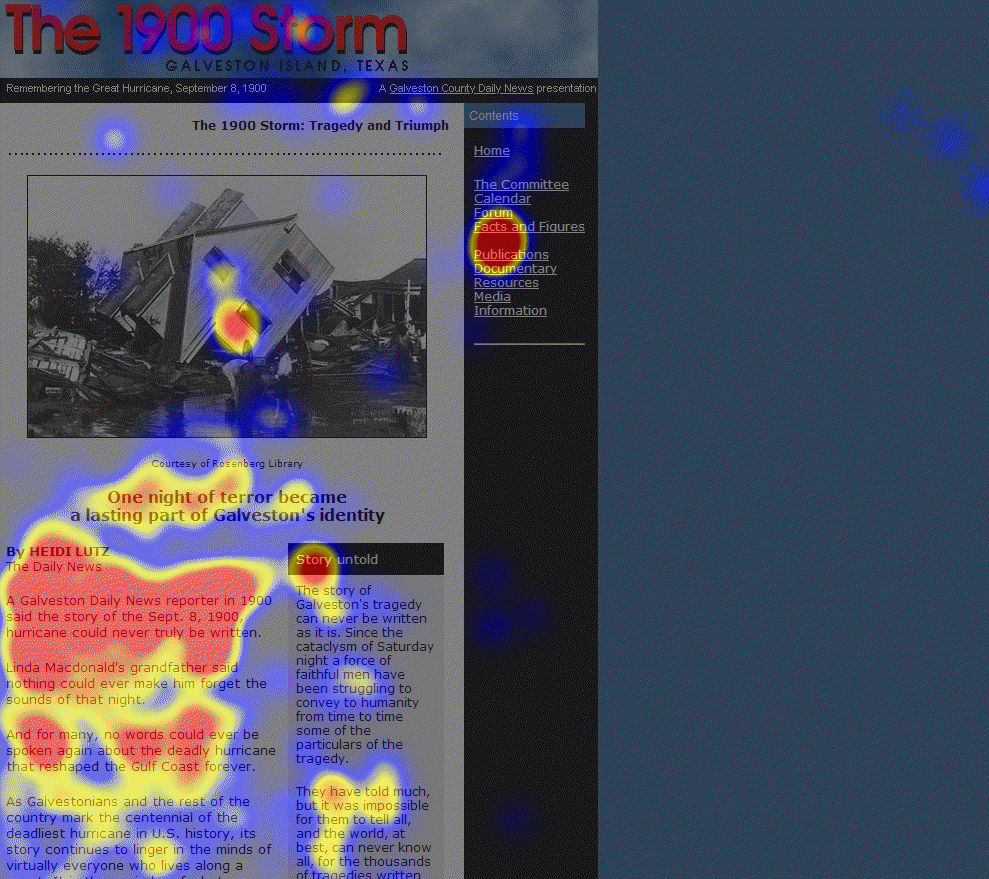
\includegraphics[width=0.6\textwidth]{tracking.png}
    \caption{Carte de chaleur d'oculométrie (\textit{heatmap}) illustrant le modèle de lecture en F identifié par le Nielsen Norman Group \cite{nielsen_fpattern_2017}. Image adaptée. Les zones rouges indiquent une fixation visuelle intense concentrée dans le coin supérieur gauche, justifiant le placement stratégique des éléments de navigation sur les bords supérieur et gauche de l’interface.}
    \label{fig:f_pattern}
\end{figure}

En conclusion, l’IU du projet \textit{Vora} constitue une application de principes issus de la psychologie cognitive, des mathématiques statistiques et de la programmation interactive, tout en prenant en compte les comportements humains. Son efficacité réside dans sa capacité à transformer des données brutes en représentations structurées et intuitives. Alors que l’arrière-plan utilise des algorithmes et du filtrage mathématique pour obtenir des données fiables, l’IU rend ces informations utiles et compréhensibles afin de réaliser l’objectif premier du projet : prévenir la sécheresse oculaire.

% ANALYSE ET DISCUSSION
\newpage
\section{Analyse et discussion}

L'objectif principal de ce projet consistait à concevoir un logiciel capable de détecter la fatigue oculaire chez l'utilisateur par une analyse de la fréquence de ses clignements d'yeux. Cette étape de détection a été accomplie avec succès, permettant au système d'identifier les clignements pour tout utilisateur situé devant un ordinateur. Comme exposé dans les recherches individuelles et dans la description du projet, la précision atteinte rend les erreurs logicielles rares et presque négligeables quant à la fiabilité globale du système. 

\begin{figure}[H]
     \centering
     \begin{subfigure}[b]{0.48\textwidth}
         \centering
         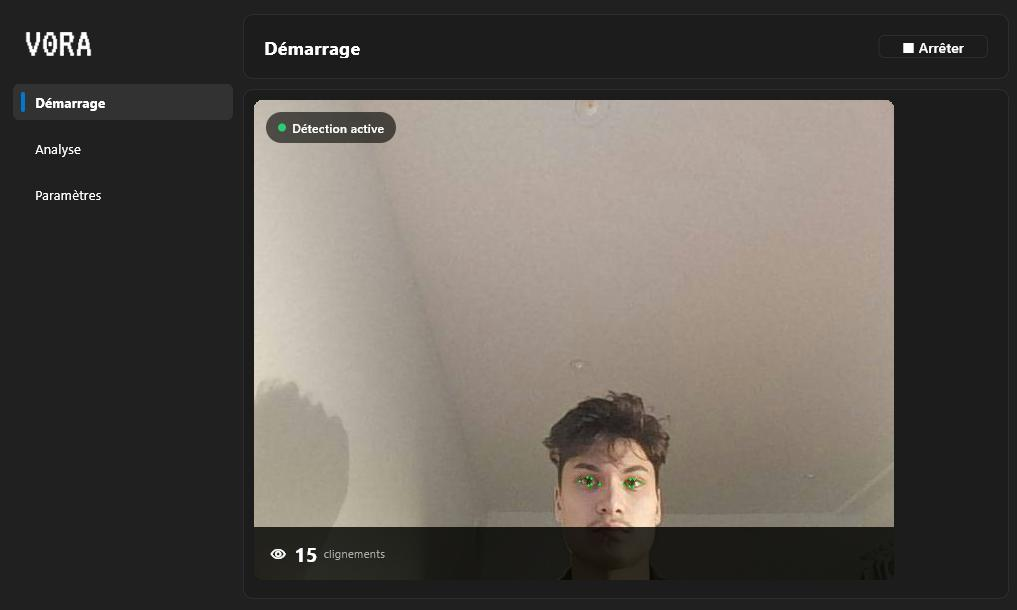
\includegraphics[width=\textwidth]{main_interface.jpg}
         \caption{Interface de démarrage et détection}
         \label{fig:interface_demarrage}
     \end{subfigure}
     \hfill
     \begin{subfigure}[b]{0.48\textwidth}
         \centering
         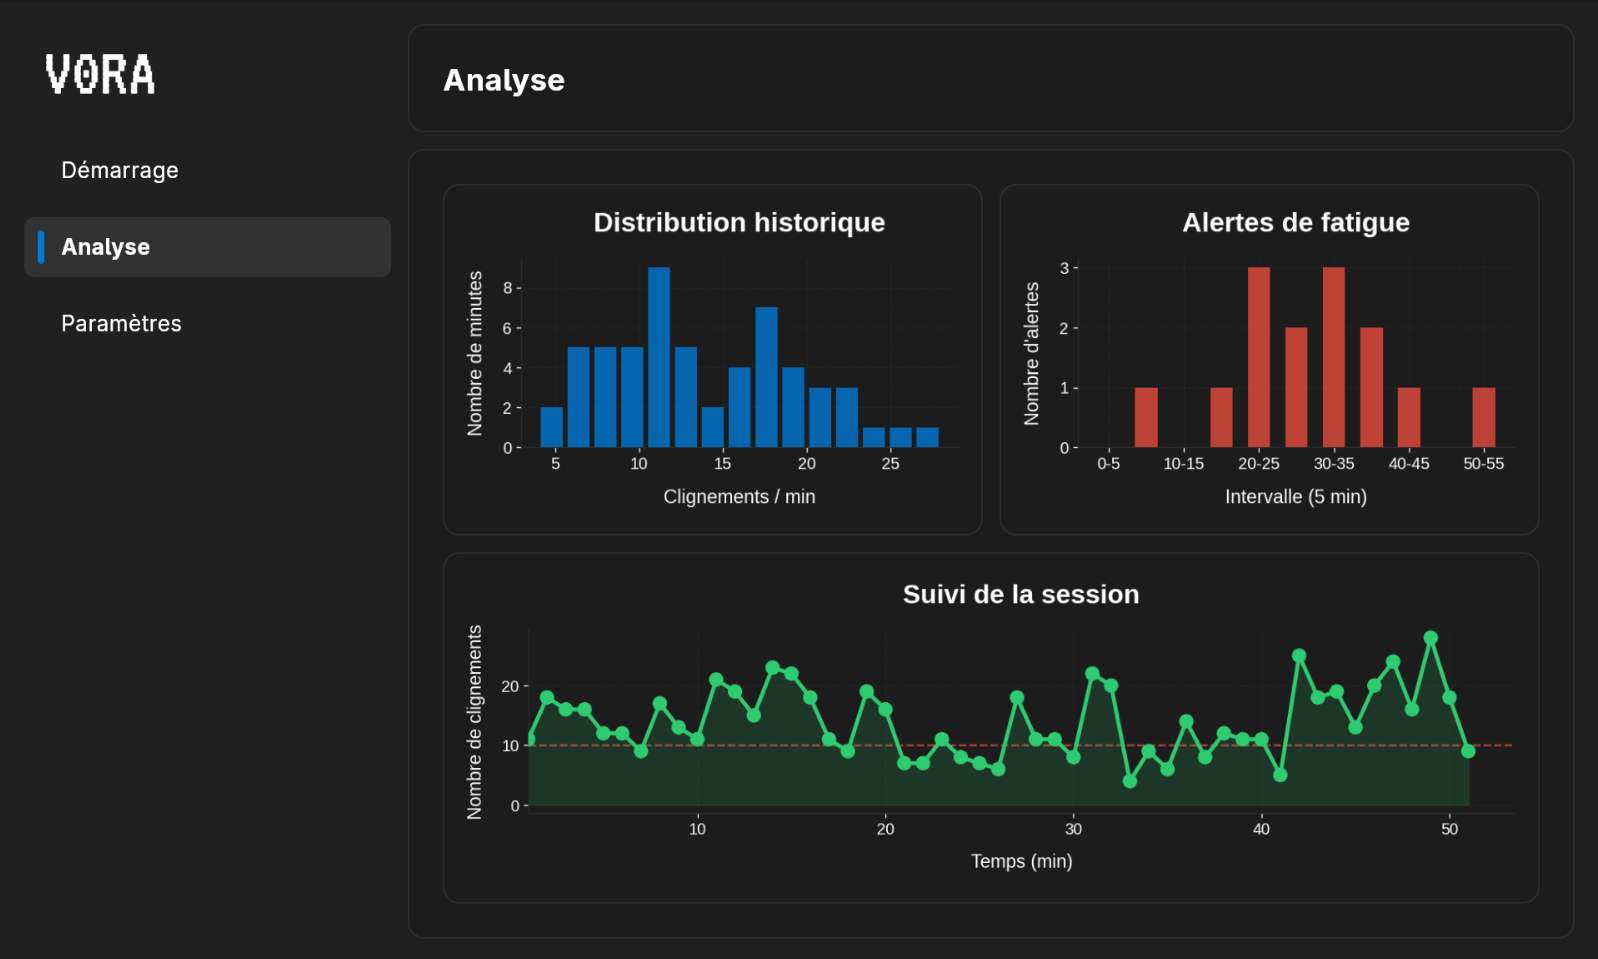
\includegraphics[width=\textwidth]{graphics.png}
         \caption{Tableau de bord et analyses}
         \label{fig:interface_analyse}
     \end{subfigure}
     \caption{Aperçu de l'interface utilisateur de Vora}
     \label{fig:ui_vora}
\end{figure}

Cependant, bien que les erreurs de détection soient peu fréquentes, le logiciel demeure tributaire de la performance de la bibliothèque MediaPipe. Puisque cette bibliothèque assure l'intégralité de la détection des points faciaux, il existe une dépendance directe envers sa capacité réelle à localiser ces repères. Bien que Google ait entraîné ce modèle sur plus de 30~000 images imparfaites pour réduire le bruit et les erreurs de détection, la bibliothèque présente certains défauts susceptibles d'induire des erreurs logicielles.

En premier lieu, la précision de l'extraction des points faciaux diminue en environnement sombre. Dans l'obscurité, le capteur de la caméra applique un gain au signal électrique capté par chaque pixel. Alors qu'en plein jour les signaux sont clairs et forts, l'absence de photons en milieu sombre force la caméra à amplifier artificiellement le signal reçu pour produire une image. Ce processus amplifie simultanément le bruit numérique, créant une texture granuleuse. Le réseau de neurones chargé d'identifier les points du visage est alors limité par ce bruit, ce qui génère des données instables pouvant empêcher le calcul de l'indice d'ouverture de l'œil (\textit{EAR}). Par conséquent, la détection est limitée non seulement par la qualité du matériel optique, mais aussi par la difficulté de MediaPipe à fournir des données stables sous faible éclairage.

De plus, le temps d'exposition de la caméra en milieu obscur introduit un flou de mouvement (« \textit{motion blur} »). En plein jour, la caméra effectue des captures ultra-rapides, tandis que dans l'obscurité, elle augmente le temps de pose pour capter davantage de lumière. Le clignement étant l'un des mouvements les plus rapides du corps humain, l'augmentation du temps d'exposition rend le calcul et la détection de ces événements beaucoup plus complexes. Ces contraintes matérielles et logicielles dictent donc les limites de précision du logiciel dans des conditions non optimales.

Un modèle tel que MediaPipe, bien qu'entraîné sur une vaste base de données, peut présenter des variations de précision selon la morphologie faciale. En effet, les travaux de David Leslie pour l'Alan Turing Institute démontrent que les annotateurs humains, en plaçant manuellement les points de repère sur les yeux, introduisent des biais inconscients. Ces erreurs d'étiquetage (\textit{labeling}), influencées par la morphologie ou l'origine ethnique des visages observés, sont par la suite assimilées par l'intelligence artificielle. Ce phénomène est susceptible de fausser la détection des mouvements oculaires si la physionomie de l'utilisateur ne correspond pas aux normes subjectives des annotateurs \cite{leslie2020understanding}.

% Paragraphe sur le UI et le scaling de la caméra (À rajouter ultérieurement)

Concernant la détection de la fatigue, plusieurs limites sont également identifiées. Le système s'appuie sur un seuil empirique de la fréquence de clignements par minute issu de la littérature scientifique. Selon l'étude \textit{Dry Eyes and Video Display Terminals} publiée par Tsubota dans le \textit{New England Journal of Medicine}, le taux moyen de clignements passe de 22/min. à une valeur comprise entre 7 et 10/min. lors d'un travail sur écran \cite{tsubota1993dryeyes}. Un seuil de fatigue fixé à 10 clignements par minute a donc été retenu. Un passage sous ce seuil est considéré comme un indicateur fort de risque de sécheresse et de fatigue visuelle.

Toutefois, cette étude repose sur un échantillon de 104 employés de bureau au Japon. Par conséquent, le logiciel ne s'adapte pas spécifiquement aux particularités physiologiques de chaque utilisateur. Une solution consisterait à implémenter un modèle d'apprentissage autonome capable de s'ajuster à l'utilisateur et à sa progression en tenant compte de facteurs tels que le moment de la journée, le type d'activité informatique, l'âge ou le sexe. En somme, l'utilisation exclusive d'une fréquence fixe limite la capacité à détecter la fatigue avec une précision absolue, celle-ci dépendant d'une multitude de facteurs dynamiques.

% CONCLUSION
\newpage
\section{Conclusion}

Après plusieurs semaines de travail, le projet \textit{Vora} est désormais capable de détecter les yeux et leurs clignements, d’enregistrer les données dans un fichier local et d’alerter l’utilisateur si le nombre de clignements est sous le seuil ou si une présence de vingt minutes devant l’écran est détectée. Pour être plus précis, les résultats montrent que l’approche combinant l’\textit{Eye Aspect Ratio} (\textit{EAR}) ainsi que l’utilisation de moyennes mobiles permet d’améliorer la stabilité des données en éliminant les faux positifs et les faux négatifs, ce qui permet une analyse fiable. 

Ces fonctionnalités sont intégrées dans une interface graphique pouvant afficher la caméra et les données recueillies, traitées sous forme de graphiques. Sachant que le but était de concevoir un assistant pouvant détecter et prévenir la fatigue oculaire, l’objectif a été atteint. 

Cependant, certaines limites demeurent. Les tests montrent que, même si dans la plupart des cas les données sont correctes, la précision diminue lorsque la luminosité est trop faible ou que la qualité de la caméra est insuffisante. Cela s’explique par le fonctionnement de la bibliothèque MediaPipe, tel que détaillé dans la section d'analyse. De plus, le modèle se base sur des études qui généralisent l’information (notamment le seuil de clignement situé entre 10 et 15) et non sur un modèle personnalisé pour chaque utilisateur. 

À travers le projet \textit{Vora}, une autre problématique liée à l’augmentation des interactions prolongées avec les écrans peut être observée. Plusieurs études montrent qu’il existe une corrélation entre le temps passé devant un écran et le risque de dépression et d’anxiété. Dans un monde où la technologie prend de plus en plus de place, la question de l’impact de ces technologies ne se limite plus aux effets physiques, mais s’étend également aux effets psychologiques \cite{li2022depression}. 

Afin de répondre à cette problématique, \textit{Vora} pourrait évoluer vers un système d’assistance plus général. À travers la combinaison de la vision par ordinateur et de l’analyse comportementale, il serait possible de surveiller non seulement la santé oculaire, mais aussi certains indicateurs liés au bien-être mental, créant ainsi un système capable de participer activement au bien-être global de l’utilisateur. Bien évidemment, certains ajouts doivent être faits afin que \textit{Vora} puisse être utilisé par le grand public, comme l'exportation de l’application vers un format exécutable avec un installateur simplifié, le portage sur mobile et la création d’un modèle d’apprentissage autonome permettant de s’adapter à chaque utilisateur.

% BIBLIOGRAPHIE
\newpage
\nocite{girard2026vora}
\printbibliography

% ANNEXE
\newpage
\pagestyle{fancy}
\fancyhf{}
\renewcommand{\headrulewidth}{0pt}
\fancyfoot[C]{A-\arabic{page}}  % → "A-16", "A-17", etc.

\begin{sidewaysfigure}
\section{Annexe}

\renewcommand{\arraystretch}{2}
\begin{tabular}{
  >{\bfseries}p{4.8cm}
  >{\centering\arraybackslash}p{3.2cm}
  >{\arraybackslash}p{31em}
}
\toprule
\textbf{Section} &
\textbf{Responsable} &
\textbf{Détail des contributions} \\

\toprule
Résumé & Arthur & Rédaction du résumé expliquant en grandes lignes le projet. \\ 
Introduction & Arthur & Problématique, revue de littérature approfondie, rappel des objectifs.\\
Description du\newline projet & Arthur,\newline François, Maxime & Explications sur le programme (Arthur), logique globale du code (Arthur) et rappel de qui a fait quoi (Arthur, François, Maxime). \\
Efficacité du\newline filtre DoMA & Arthur & Question de recherche portant sur les filtres dans le large domaine du traitement de signal. \\
Fonctionnement de\newline MediaPipe & François & Question de recherche portant sur le réseau de neurones derrière MediaPipe et son fonctionnement. \\
Interface graphique\newline et le cognitif & Maxime & Question de recherche portant sur le dessin d'interfaces graphiques en informatique. \\
Résultats et\newline discussion & François,\newline Maxime & Interprétation des résultats (François), comparaisons à la littérature (François), analyse des limites du projet (François, Maxime).  \\
Conclusion & Maxime & Rappel des résultats clés, ouverture, approfondissements possibles.\\
Références & Arthur & Intégration des citations sous format IEEE dans \LaTeX\ avec l'aide de BibTex.\\
\bottomrule
\end{tabular}

\end{sidewaysfigure}
\end{document}
